\documentclass[12pt,a4paper]{article}
\usepackage[utf8]{inputenc}
\usepackage[T1]{fontenc}
\usepackage[english]{babel}
\usepackage{geometry}
\usepackage{booktabs}
\usepackage{array}
\usepackage{enumitem}
\usepackage{hyperref}
\usepackage{xcolor}
\usepackage{titlesec}
\usepackage{parskip}
\usepackage{amssymb}
\usepackage{graphicx}
\graphicspath{{}}
\usepackage{tikz}
\usetikzlibrary{shapes.geometric, arrows.meta, positioning}

\geometry{margin=2.5cm}

\hypersetup{
    colorlinks=true,
    linkcolor=black,
    urlcolor=blue
}

\titleformat{\section}{\large\bfseries}{}{0em}{}[\titlerule]
\titleformat{\subsection}{\normalsize\bfseries}{}{0em}{}

\title{
    \textbf{WorkFlow}\\
    \large Field Team Coordination App\\[0.5em]
    \normalsize Project Documentation
}
\author{Adam Strelec \and Damián Styrak}
\date{February 2026}

\begin{document}

\maketitle
\tableofcontents
\newpage

%--------------------------------------------------------------
\section{Application Overview}
%--------------------------------------------------------------

\textbf{WorkFlow} is a cross-platform mobile application (iOS / Android) designed
for coordinating field work teams. It replaces inefficient phone- or email-based
coordination by giving managers an instant, real-time overview of task progress and
team locations.

\textbf{Core features:}
\begin{itemize}[noitemsep]
    \item Creating, editing, and assigning projects and tasks within them to field workers.
    \item Live tracking of worker GPS positions on an interactive map.
    \item Task status updates and photo documentation upload directly from the field.
    \item Built-in real-time chat (WebSocket) between managers and workers.
    \item Push notifications for new assignments and status changes.
    \item Offline mode --- changes are saved locally and synced automatically on reconnect.
\end{itemize}

\subsection*{Technology Stack}

\begin{center}
\begin{tabular}{ll}
\toprule
\textbf{Layer} & \textbf{Technology} \\
\midrule
Frontend           & React Native (iOS / Android) \\
Backend            & Node.js (Express) \\
Database           & PostgreSQL \\
Push notifications & FCM (Android) + APNs via FCM (iOS) \\
Authentication     & Google SSO (OAuth 2.0) \\
Maps               & react-native-maps (Google Maps / Apple Maps) \\

\bottomrule
\end{tabular}
\end{center}

%--------------------------------------------------------------
\section{User Roles}
%--------------------------------------------------------------

The application defines two user roles with distinct permissions.

\subsection{Manager}

The Manager has full control over projects, tasks, and the team:
\begin{itemize}[noitemsep]
    \item Creates, edits, and deletes projects.
    \item Creates, edits, and deletes tasks within projects (title, description, GPS coordinates, deadline).
    \item Assigns tasks to one or more workers.
    \item Views live worker positions and task-site pins on the map.
    \item Has an overview of all tasks and their current statuses.
    \item Reviews and accepts worker skill certificates.
    \item Communicates with workers via the built-in chat.
    \item Receives a push notification when a worker marks a task as \textit{Done}.
\end{itemize}

\subsection{Worker}

The Worker has restricted access --- only to tasks assigned to them:
\begin{itemize}[noitemsep]
    \item Views the list of their assigned tasks.
    \item Opens task details: description, map, photos, current status.
    \item Changes the task status to \textit{In Progress} or \textit{Done}.
    \item Uploads photo documentation from the camera or gallery.
    \item Uploads skill certificates for manager review.
    \item Shares GPS location with the manager (every 10 seconds).
    \item Communicates with the manager via chat.
    \item Receives a push notification when a new task is assigned.
    \item Can update task status offline; the change syncs after reconnection.
\end{itemize}


%--------------------------------------------------------------
\section{Screen Design}
%--------------------------------------------------------------

The application contains the following functional screens (splash and login screens
are not counted). Screens differ in available actions depending on the user role.

\subsection{Screen 1 --- Dashboard (Manager)}

\textbf{Description:} The home screen for the Manager after login. Provides a quick
summary of the current state of all work.

\textbf{UI elements:}
\begin{itemize}[noitemsep]
    \item Manager name, role badge, and online status.
    \item Summary card showing active vs.\ total tasks (e.g.\ 4/13 active, 9/13 pending) with a \textbf{Detail} button.
    \item Summary card showing total number of workers with a \textbf{Detail} button.
    \item Bottom navigation bar: Profile, Home, Chat.
\end{itemize}

\subsection{Screen 2 --- Project List}

\textbf{Description:} List of all projects. Manager sees an \textbf{Add project +} button;
workers see only projects they are assigned to.

\textbf{UI elements:}
\begin{itemize}[noitemsep]
    \item Scrollable list of projects, each with name and navigation arrow.
    \item \textbf{Add project +} button in the top right (Manager only).
    \item Tap a project --- navigates to Project Detail.
\end{itemize}

\subsection{Screen 3 --- Project Detail}

\textbf{Description:} Full detail view of a project. The layout differs by role.

\textbf{UI elements (Manager):}
\begin{itemize}[noitemsep]
    \item Project title, status, deadline, location, created by, created at.
    \item Client info: name, phone, email, construction site address.
    \item Progress section: tasks done counter (e.g.\ 3/7) and number of assigned workers.
    \item List of assigned workers with online/offline status indicators.
    \item Photo documentation gallery with \textbf{+} button to add photos.
    \item Action buttons: \textbf{Edit project}, \textbf{Delete project}, \textbf{Assign worker}, \textbf{Add task}, \textbf{View map}.
\end{itemize}

\textbf{UI elements (Worker):}
\begin{itemize}[noitemsep]
    \item Project title, status, deadline, location, created by.
    \item Client name and phone.
    \item Progress bar showing percentage of tasks completed.
    \item Tasks done counter with navigation to task list.
    \item Photo documentation gallery with \textbf{+} button.
\end{itemize}

\subsection{Screen 4 --- Project Creation}

\textbf{Description:} Form for creating a new project. Available to Manager only.

\textbf{UI elements:}
\begin{itemize}[noitemsep]
    \item Project info: Title, Description, Deadline, Status (radio button).
    \item Location: Construction site address, GPS Latitude, GPS Longitude.
    \item Client info: Client name, Phone, Email.
    \item \textbf{Save} button.
\end{itemize}

\subsection{Screen 5 --- Task List}

\textbf{Description:} List of tasks within a project. Accessible from Project Detail.

\textbf{UI elements:}
\begin{itemize}[noitemsep]
    \item Project name in the header.
    \item Filter icon and \textbf{+} button (Manager only) to add a new task.
    \item Expandable task cards showing: title, status indicator, category, description, assigned person, deadline, photo thumbnails, \textbf{Upload more photos} link, and \textbf{Mark as done} button.
    \item Collapsed tasks show only title and status.
\end{itemize}

\subsection{Screen 6 --- Task Creation}

\textbf{Description:} Form for creating a new task within a project. Manager only.

\textbf{UI elements:}
\begin{itemize}[noitemsep]
    \item Title and Description fields.
    \item Category dropdown (e.g.\ Elektrika, Kurenie) and Deadline picker.
    \item Priority selector: Low / Medium / High.
    \item Assign worker section --- shows available workers with their verified skill certificates.
    \item \textbf{Save Task} button.
\end{itemize}

\subsection{Screen 7 --- Assign Worker}

\textbf{Description:} Screen for assigning a worker to a task. Manager only.

\textbf{UI elements:}
\begin{itemize}[noitemsep]
    \item Search bar for filtering workers.
    \item Skill filter chips (e.g.\ All, Elektrika, Voda, Kurenie, Plyn).
    \item \textit{Available workers} section --- each card shows name and verified skill badges; selectable via checkbox.
    \item \textit{Missing certificate --- not eligible} section showing workers who cannot be assigned due to missing qualifications.
    \item \textbf{Done} button to confirm assignment.
\end{itemize}

\subsection{Screen 8 --- Map}

\textbf{Description:} Project-specific map showing live worker positions. Manager only.

\textbf{UI elements:}
\begin{itemize}[noitemsep]
    \item Project name in the header (e.g.\ \textit{Project1 map}).
    \item Full-screen map view with worker markers.
    \item \textit{Workers on this project} section below the map listing each worker with name and online/offline status.
\end{itemize}

\subsection{Screen 9 --- Chat}

\textbf{Description:} Direct real-time messaging between Manager and Worker.

\textbf{UI elements:}
\begin{itemize}[noitemsep]
    \item Header with recipient's name, avatar, and online status.
    \item Message history in chronological order (alternating left/right alignment).
    \item Chat input field and \textbf{Send} button.
\end{itemize}

\subsection{Screen 10 --- Worker List}

\textbf{Description:} Manager's overview of all their workers.

\textbf{UI elements:}
\begin{itemize}[noitemsep]
    \item Expandable worker cards --- expanded view shows verified and missing skill certificates (e.g.\ Voda \checkmark, Kurenie \texttimes).
    \item \textbf{Viac} (More) link for additional certificates.
    \item \textbf{Invite new worker} button at the bottom --- generates a unique invite link (e.g.\ \texttt{workflow://invite?token=...}) that can be copied and shared.
\end{itemize}

\subsection{Screen 11 --- Worker Profile (Manager view)}

\textbf{Description:} Manager's view of a worker's profile.

\textbf{UI elements:}
\begin{itemize}[noitemsep]
    \item Profile photo, first name, last name, hourly rate.
    \item List of skill categories with certificate status (verified / not verified) and \textbf{Zobraziť} (Show) link per certificate.
\end{itemize}

\subsection{Screen 12 --- Profile (Worker view)}

\textbf{Description:} Worker's own profile and settings.

\textbf{UI elements:}
\begin{itemize}[noitemsep]
    \item Profile photo, username, last name, date of birth, hourly rate, bank information.
    \item \textbf{Edit profile} button.
    \item List of skill categories with certificate status.
    \item \textbf{Log out} button.
\end{itemize}

\subsection{Screen 13 --- Certificates (Worker --- Send)}

\textbf{Description:} Screen for uploading a skill certificate for manager review.

\textbf{UI elements:}
\begin{itemize}[noitemsep]
    \item Informative text about the certificate request.
    \item Sender name label.
    \item Large photo upload area with \textbf{+} button (camera or gallery).
\end{itemize}

\subsection{Screen 14 --- Certificates (Manager --- Review)}

\textbf{Description:} Screen for reviewing a certificate submitted by a worker.

\textbf{UI elements:}
\begin{itemize}[noitemsep]
    \item Informative text and sender name.
    \item Certificate photo preview.
    \item \textbf{Accept} (\checkmark) and \textbf{Reject} (\texttimes) action buttons.
\end{itemize}

%--------------------------------------------------------------
\section{Prototype}
%--------------------------------------------------------------

\subsection*{Navigation Flow}

The app uses a \textbf{bottom tab bar} (Profile, Home, Chat) for top-level navigation
and \textbf{stack navigation} within each section.

\begin{center}
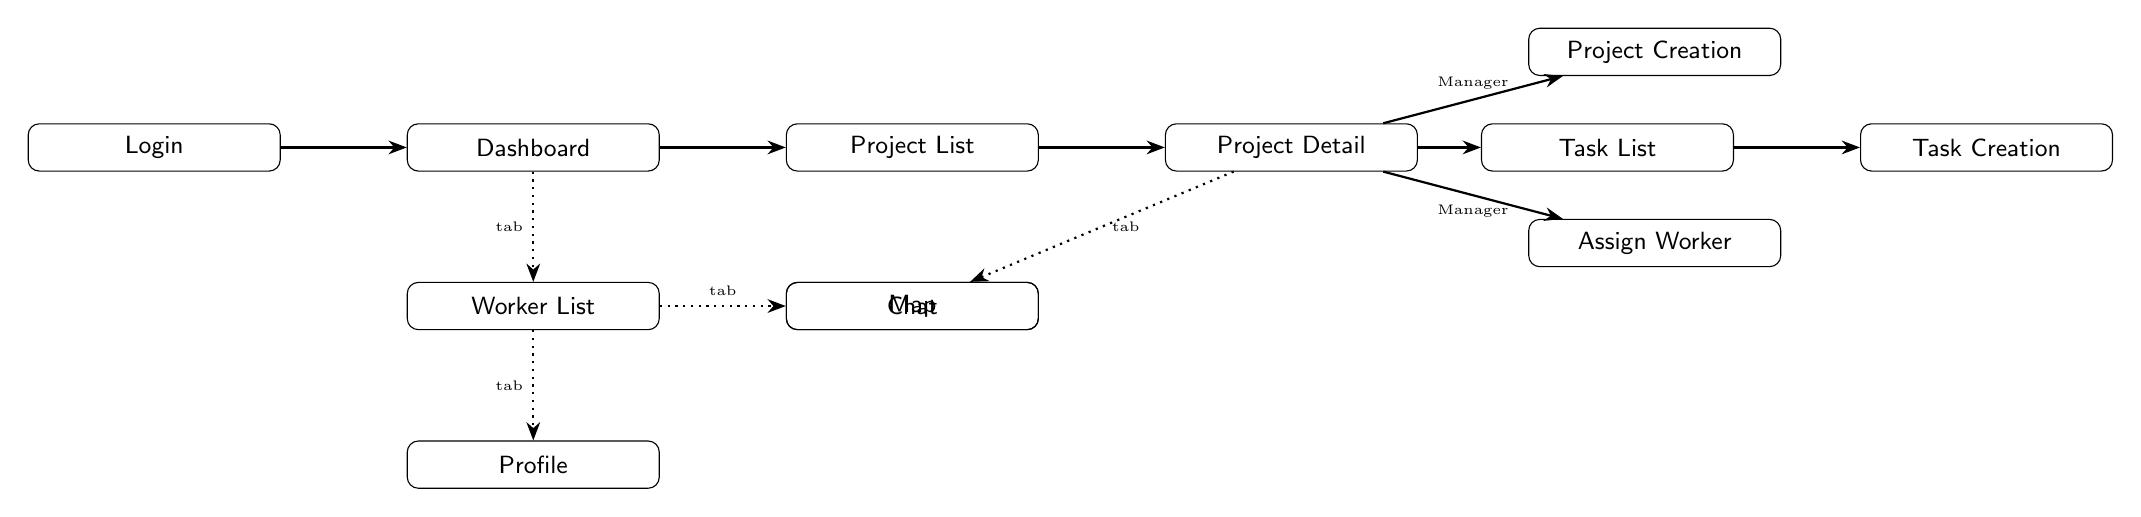
\begin{tikzpicture}[
    node distance=0.9cm and 1.6cm,
    box/.style={draw, rounded corners, minimum width=3.2cm, minimum height=0.6cm,
                font=\small\sffamily, align=center},
    arr/.style={-{Stealth}, thick},
    tab/.style={-{Stealth}, thick, dotted}
]
\node[box] (login)    {Login};
\node[box, right=of login]   (dash)    {Dashboard};
\node[box, right=of dash]    (plist)   {Project List};
\node[box, right=of plist]   (pdetail) {Project Detail};

\node[box, above right=0.6cm and 1.4cm of pdetail] (pcreate) {Project Creation};
\node[box, right=0.8cm of pdetail]                 (tlist)   {Task List};
\node[box, below right=0.6cm and 1.4cm of pdetail] (assign)  {Assign Worker};

\node[box, right=of tlist]   (tcreate) {Task Creation};
\node[box, below=1.4cm of plist]  (map)     {Map};
\node[box, below=1.4cm of dash]   (wlist)   {Worker List};
\node[box, below=1.4cm of wlist]  (profile) {Profile};
\node[box, right=of wlist]        (chat)    {Chat};

\draw[arr] (login)   -- (dash);
\draw[arr] (dash)    -- (plist);
\draw[arr] (plist)   -- (pdetail);
\draw[arr] (pdetail) -- node[above,font=\tiny]{Manager} (pcreate);
\draw[arr] (pdetail) -- (tlist);
\draw[arr] (pdetail) -- node[below,font=\tiny]{Manager} (assign);
\draw[arr] (tlist)   -- (tcreate);

\draw[tab] (dash)  -- node[left,font=\tiny]{tab} (wlist);
\draw[tab] (wlist) -- node[left,font=\tiny]{tab} (profile);
\draw[tab] (wlist) -- node[above,font=\tiny]{tab} (chat);
\draw[tab] (pdetail) -- node[right,font=\tiny]{tab} (map);
\end{tikzpicture}
\end{center}

\subsection*{Prototype Screens}

The following screens represent the actual designed prototype of the WorkFlow application.

\bigskip
\noindent\textbf{Dashboard \& Project List}

\begin{center}
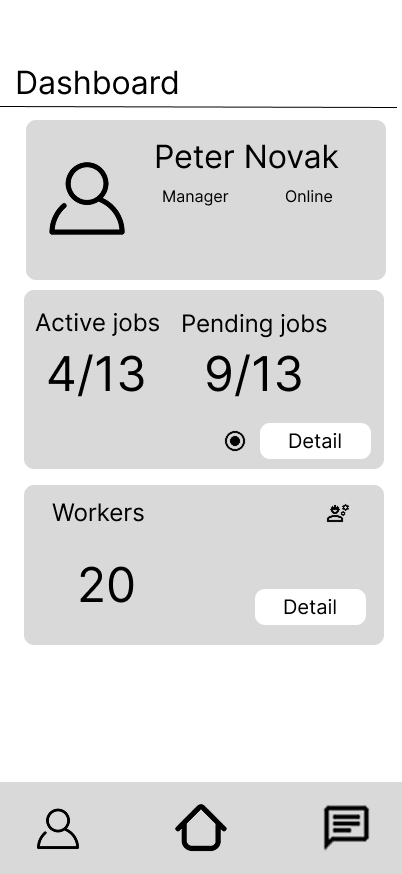
\includegraphics[width=0.28\textwidth]{Home Page - manager.png}\hspace{0.5cm}
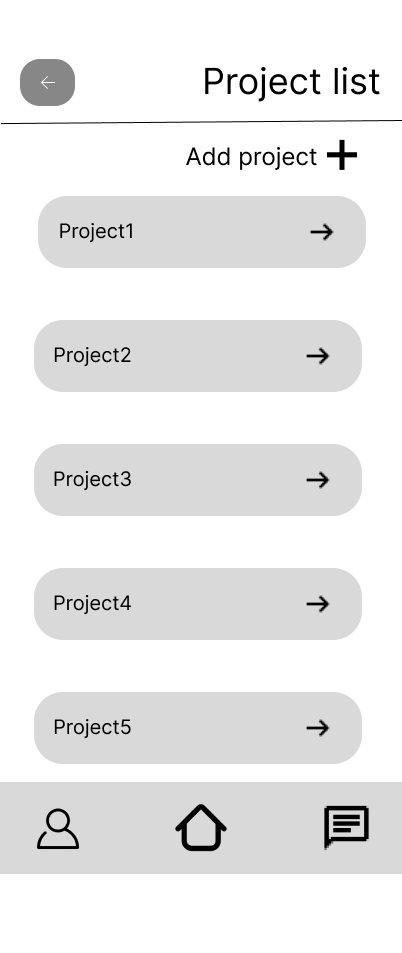
\includegraphics[width=0.28\textwidth]{Project list.png}\hspace{0.5cm}
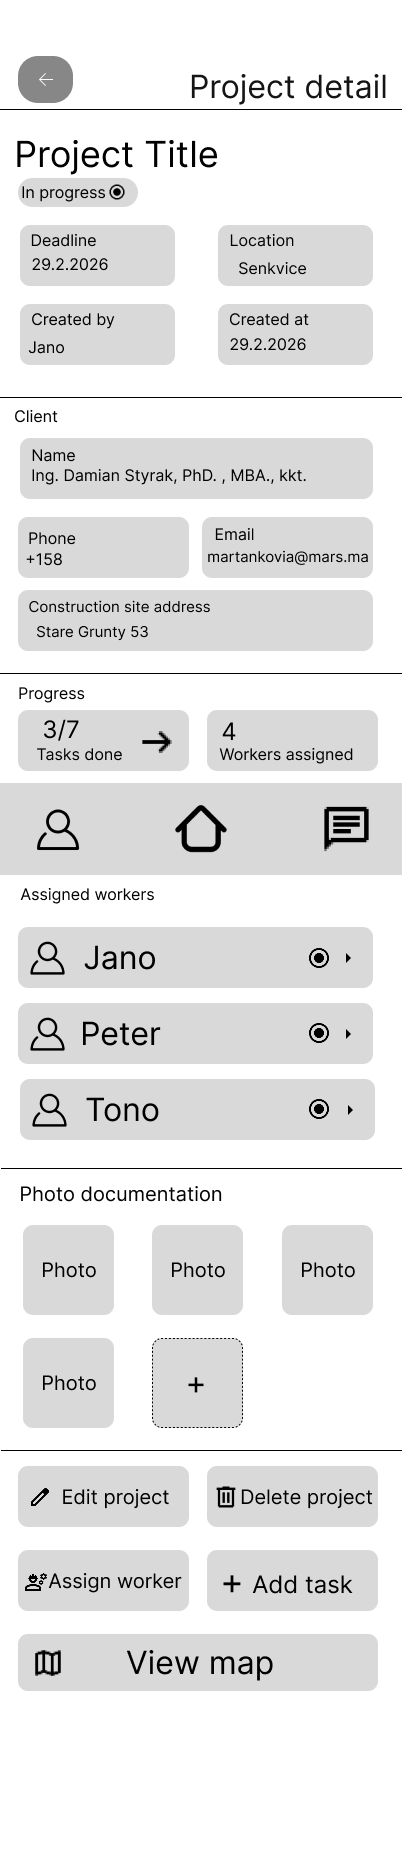
\includegraphics[width=0.28\textwidth]{Project list-pop up - manager.png}
\end{center}

\bigskip
\noindent\textbf{Project Detail (Manager \& Worker) and Project Creation}

\begin{center}
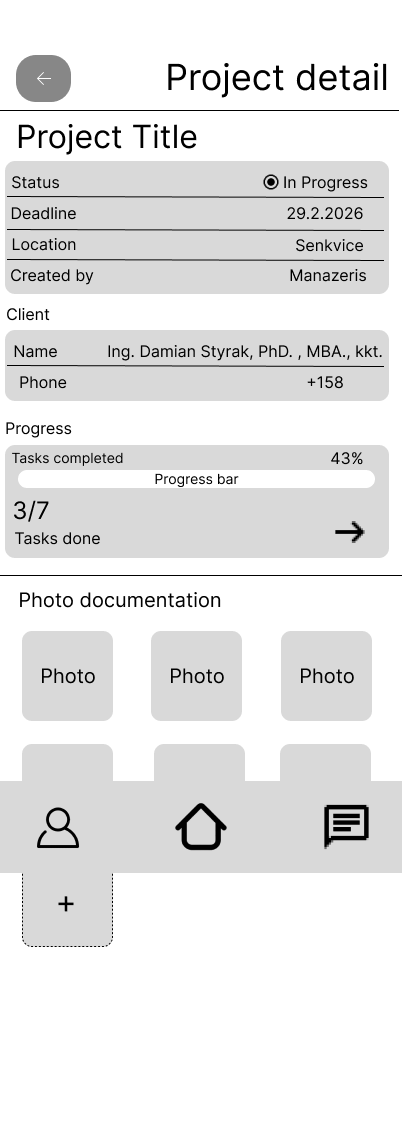
\includegraphics[width=0.28\textwidth]{Project list-pop up - worker.png}\hspace{0.5cm}
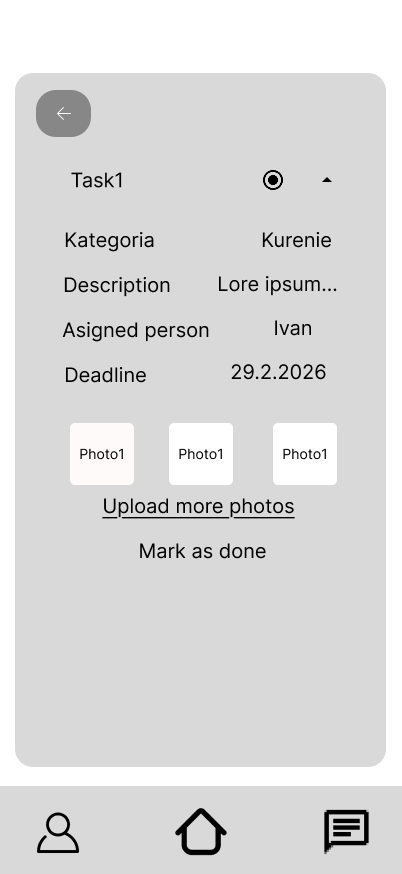
\includegraphics[width=0.28\textwidth]{Project list-pop up.png}\hspace{0.5cm}
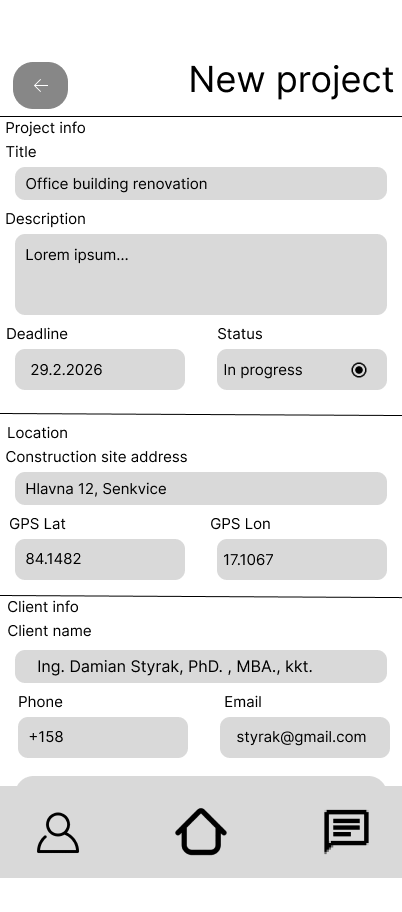
\includegraphics[width=0.28\textwidth]{Project creation.png}
\end{center}

\bigskip
\noindent\textbf{Task List, Task Detail and Task Creation}

\begin{center}
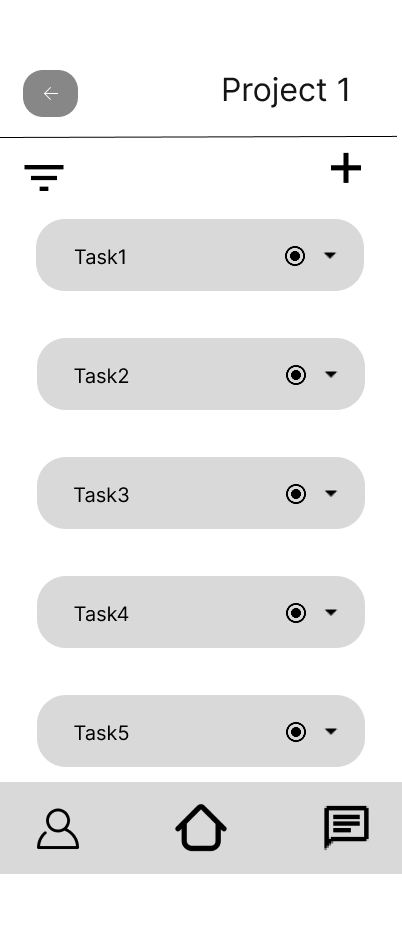
\includegraphics[width=0.28\textwidth]{Task list.png}\hspace{0.5cm}
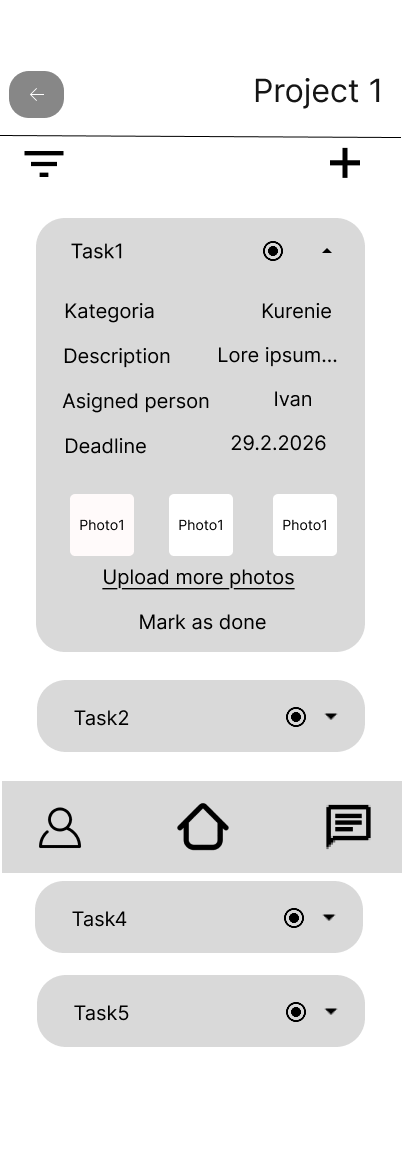
\includegraphics[width=0.28\textwidth]{Task list - detail.png}\hspace{0.5cm}
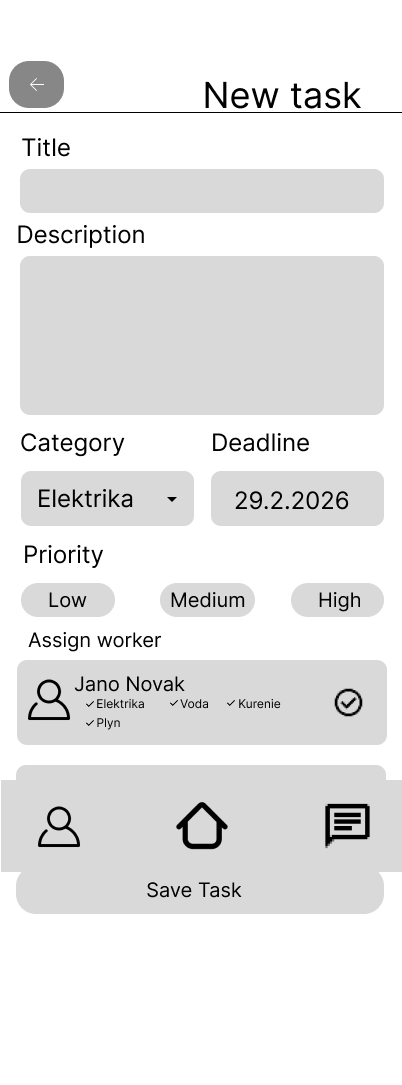
\includegraphics[width=0.28\textwidth]{Task creation.png}
\end{center}

\bigskip
\noindent\textbf{Assign Worker, Map and Chat}

\begin{center}
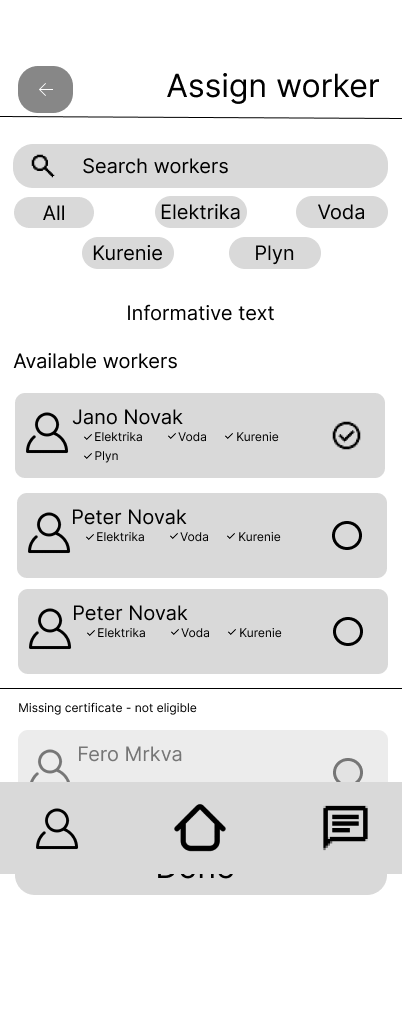
\includegraphics[width=0.28\textwidth]{Assign worker to job.png}\hspace{0.5cm}
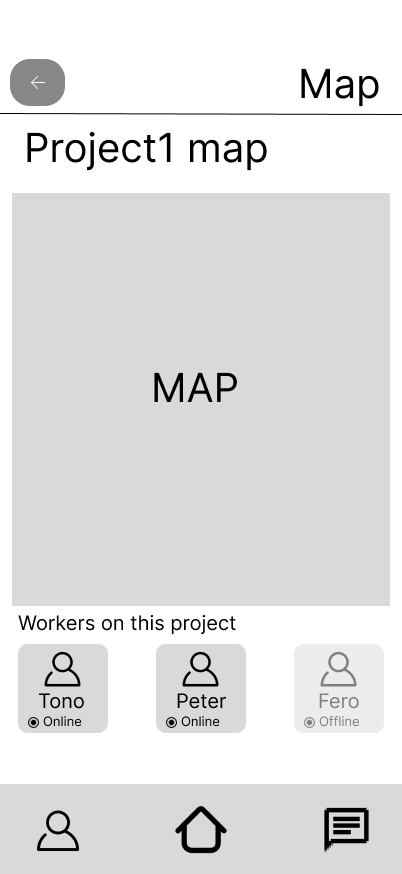
\includegraphics[width=0.28\textwidth]{Map.png}\hspace{0.5cm}
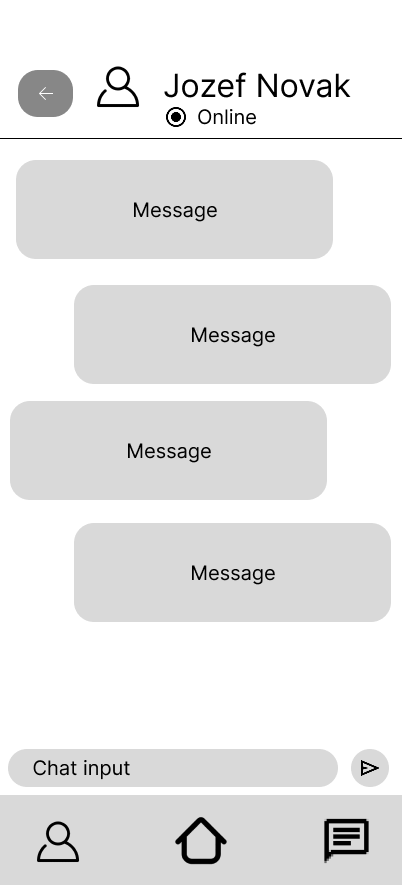
\includegraphics[width=0.28\textwidth]{Chat - detail.png}
\end{center}

\bigskip
\noindent\textbf{Worker List, Worker Detail and Invite Worker}

\begin{center}
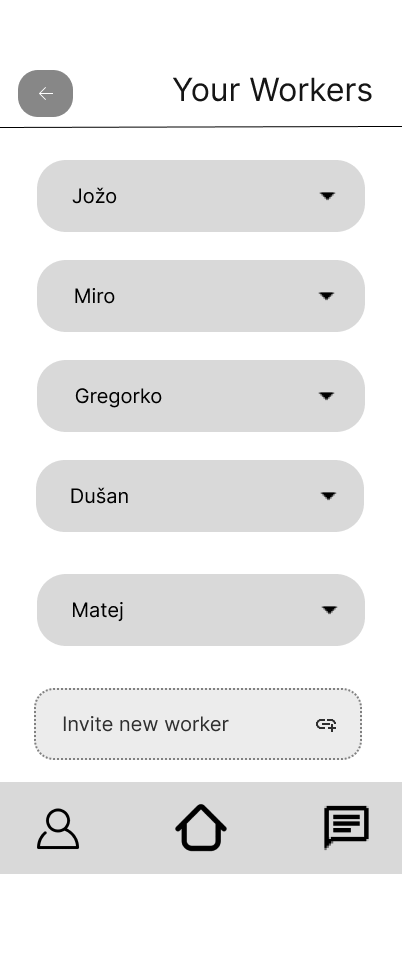
\includegraphics[width=0.28\textwidth]{Worker list.png}\hspace{0.5cm}
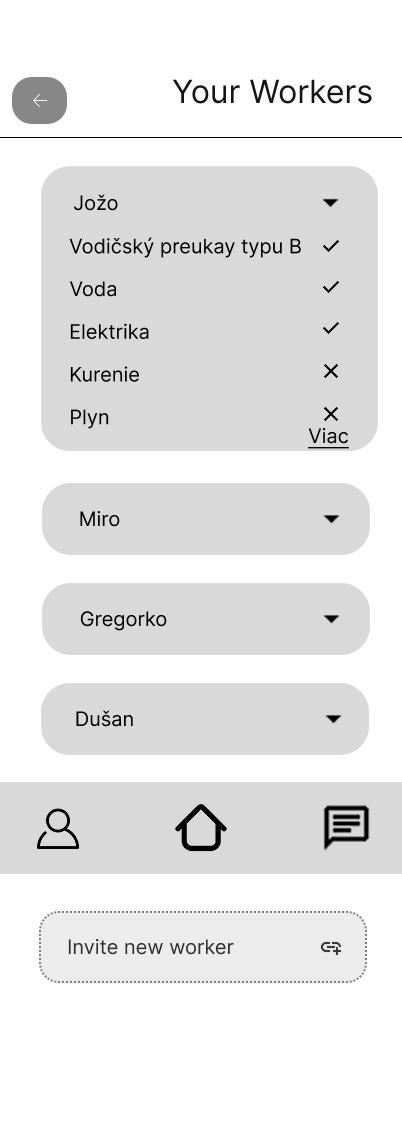
\includegraphics[width=0.28\textwidth]{Worker detail.png}\hspace{0.5cm}
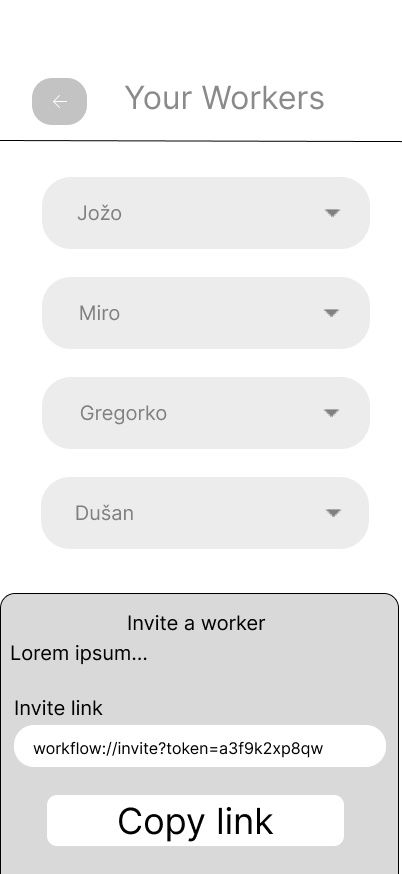
\includegraphics[width=0.28\textwidth]{Invite worker.png}
\end{center}

\bigskip
\noindent\textbf{Profiles and Certificates}

\begin{center}
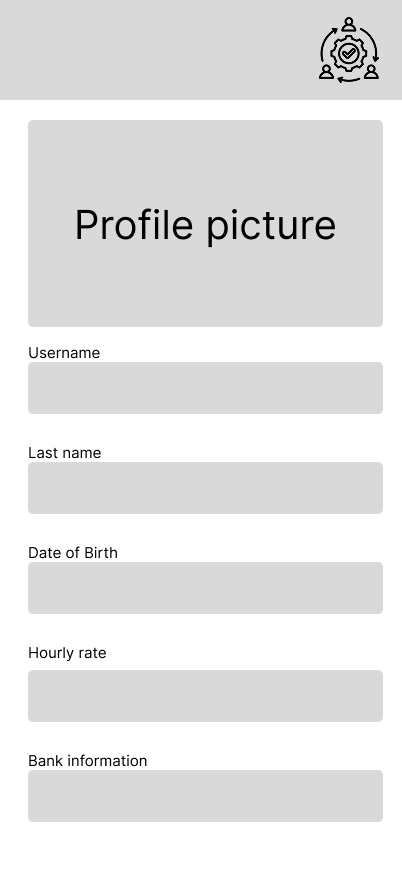
\includegraphics[width=0.28\textwidth]{Profile.png}\hspace{0.5cm}
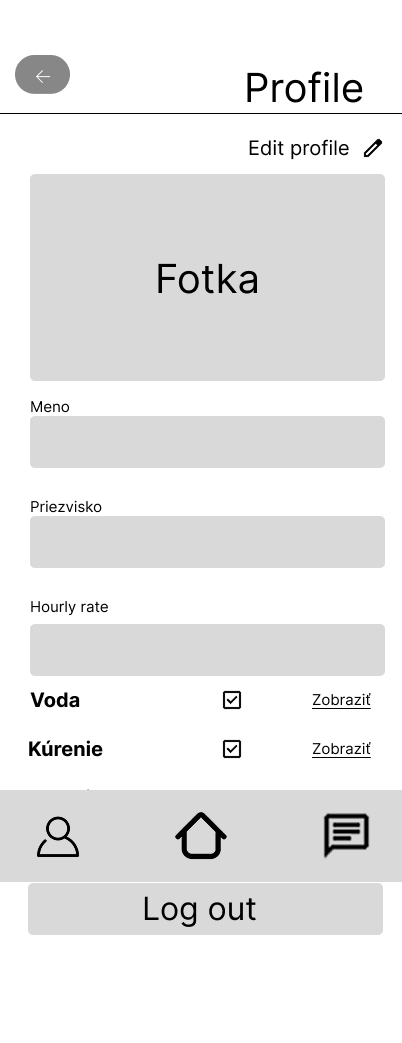
\includegraphics[width=0.28\textwidth]{Worker profile - worker - view.png}\hspace{0.5cm}
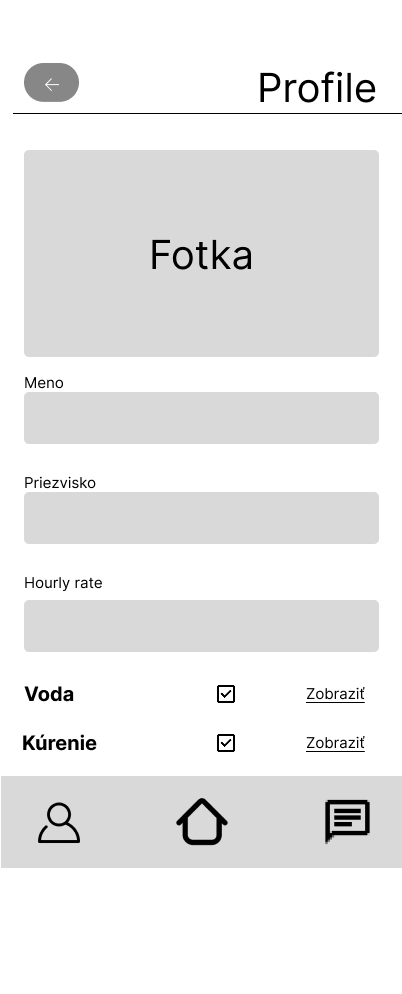
\includegraphics[width=0.28\textwidth]{Worker profile - admin.png}
\end{center}

\begin{center}
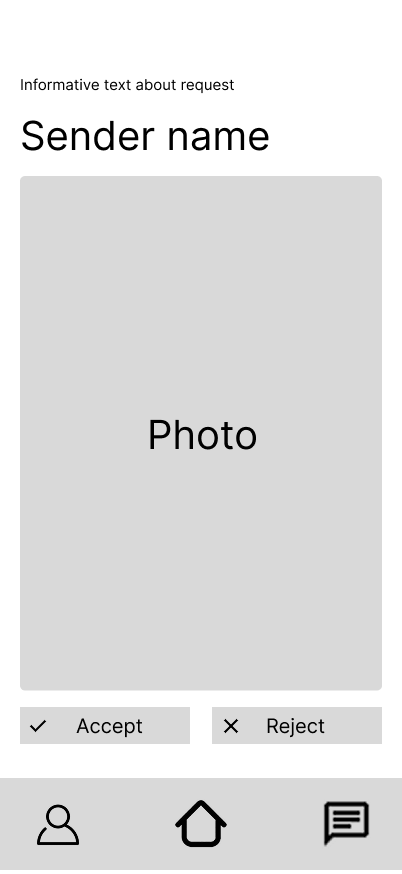
\includegraphics[width=0.28\textwidth]{Admit proof of skill - manager.png}
\end{center}


%--------------------------------------------------------------
\section{Acceptance Tests (UAT)}
%--------------------------------------------------------------

Each test contains at least 7 steps, spans at least two screens, and represents a
complete, self-contained scenario. Login and registration are not standalone UAT
scenarios.

\subsection*{Positive Tests}

\subsubsection*{UAT-01: Create a New Task}

\noindent\textbf{Preconditions:} Manager is logged in. Active internet connection.\\
\textbf{Postconditions:} The new task is saved to the database and appears in the task list.

\begin{center}
\begin{tabular}{cp{11.5cm}}
\toprule
\textbf{Step} & \textbf{Action} \\
\midrule
1 & User is on the Task List screen. \\
2 & Taps the \textbf{+} button (Create Task). \\
3 & Create Task screen appears. \\
4 & Fills in the title, description, and selects a deadline. \\
5 & Taps on the map to set the task-site location. \\
6 & Taps the \textbf{Save} button. \\
7 & App navigates back to Task List; the new task appears at the top. \\
\midrule
\textbf{Result} & PASS \quad/\quad FAIL \\
\bottomrule
\end{tabular}
\end{center}

\subsubsection*{UAT-02: Assign a Worker to a Task}

\noindent\textbf{Preconditions:} Manager is logged in. At least one Worker and one task exist.\\
\textbf{Postconditions:} Worker is assigned to the task and receives a push notification.

\begin{center}
\begin{tabular}{cp{11.5cm}}
\toprule
\textbf{Step} & \textbf{Action} \\
\midrule
1 & Manager opens Task List and taps an existing task. \\
2 & Task Detail screen is displayed. \\
3 & Taps \textbf{Assign Worker}. \\
4 & A list of workers appears; Manager selects one. \\
5 & Confirms the selection with the \textbf{Confirm} button. \\
6 & The assigned worker's name appears in Task Detail. \\
7 & Worker's device receives: \textit{``You have been assigned a new task''}. \\
\midrule
\textbf{Result} & PASS \quad/\quad FAIL \\
\bottomrule
\end{tabular}
\end{center}

\subsubsection*{UAT-03: Worker Updates Task Status}

\noindent\textbf{Preconditions:} Worker is logged in with a \textit{Pending} task. Active internet.\\
\textbf{Postconditions:} Status changes to \textit{In Progress}; Manager sees the update in real time.

\begin{center}
\begin{tabular}{cp{11.5cm}}
\toprule
\textbf{Step} & \textbf{Action} \\
\midrule
1 & Worker opens Task List (My Tasks). \\
2 & Taps a task with status \textit{Pending}. \\
3 & Task Detail screen is displayed. \\
4 & Taps the \textbf{Start Task} button. \\
5 & Confirmation dialog appears; Worker taps \textbf{Confirm}. \\
6 & Task status changes to \textit{In Progress} with the appropriate badge. \\
7 & On the Manager's device, the status updates in real time in Task List. \\
\midrule
\textbf{Result} & PASS \quad/\quad FAIL \\
\bottomrule
\end{tabular}
\end{center}

\subsubsection*{UAT-04: Upload a Photo to a Task}

\noindent\textbf{Preconditions:} Worker is logged in with an assigned task. Active internet and camera permission granted.\\
\textbf{Postconditions:} Photo is uploaded and visible in Task Detail.

\begin{center}
\begin{tabular}{cp{11.5cm}}
\toprule
\textbf{Step} & \textbf{Action} \\
\midrule
1 & Worker opens Task Detail of an assigned task. \\
2 & Scrolls to \textit{Photo Documentation} and taps \textbf{+}. \\
3 & Picker appears: \textit{Camera} or \textit{Gallery}; Worker selects \textit{Camera}. \\
4 & Camera opens; Worker takes a photo and confirms the shot. \\
5 & App uploads the photo to the server. \\
6 & A progress indicator is displayed during the upload. \\
7 & After successful upload the photo appears in the task gallery. \\
\midrule
\textbf{Result} & PASS \quad/\quad FAIL \\
\bottomrule
\end{tabular}
\end{center}

\subsubsection*{UAT-05: Real-time Chat Between Manager and Worker}

\noindent\textbf{Preconditions:} Both users are logged in with the chat of the same task open.\\
\textbf{Postconditions:} Messages appear on both devices in real time.

\begin{center}
\begin{tabular}{cp{11.5cm}}
\toprule
\textbf{Step} & \textbf{Action} \\
\midrule
1 & Manager opens Task Detail and taps \textbf{Chat}. \\
2 & Worker opens the same task and taps \textbf{Chat}. \\
3 & Manager types a message and taps \textbf{Send}. \\
4 & Message appears instantly on the Worker's device without refreshing. \\
5 & Worker replies and taps \textbf{Send}. \\
6 & Message appears instantly on the Manager's device. \\
7 & Both devices show the full history in correct chronological order. \\
\midrule
\textbf{Result} & PASS \quad/\quad FAIL \\
\bottomrule
\end{tabular}
\end{center}

\subsubsection*{UAT-06: Track Worker Location on the Map}

\noindent\textbf{Preconditions:} Manager is on Map View. Worker is logged in with location sharing active.\\
\textbf{Postconditions:} Manager sees the Worker's live position on the map.

\begin{center}
\begin{tabular}{cp{11.5cm}}
\toprule
\textbf{Step} & \textbf{Action} \\
\midrule
1 & Manager opens Map View. \\
2 & Task-site pins are visible on the map. \\
3 & Worker moves physically (or simulator changes the location). \\
4 & Worker opens the app --- GPS transmission starts. \\
5 & Worker marker appears on the Manager's map within 15 seconds. \\
6 & After further movement, the marker shifts to the new position. \\
7 & Manager taps the marker --- Worker's name and status are shown. \\
\midrule
\textbf{Result} & PASS \quad/\quad FAIL \\
\bottomrule
\end{tabular}
\end{center}

\subsubsection*{UAT-07: Offline Task Status Update}

\noindent\textbf{Preconditions:} Worker is logged in with an assigned task. No internet (airplane mode on).\\
\textbf{Postconditions:} After reconnection the status change is synced to the server.

\begin{center}
\begin{tabular}{cp{11.5cm}}
\toprule
\textbf{Step} & \textbf{Action} \\
\midrule
1 & Worker enables airplane mode. \\
2 & Opens Task List --- tasks are visible from local cache. \\
3 & Opens Task Detail and taps \textbf{Mark as Done}. \\
4 & App shows status \textit{Done} with an offline sync icon (clock). \\
5 & Worker disables airplane mode. \\
6 & App detects connectivity and triggers background sync. \\
7 & The clock icon disappears; task status is updated on the server. \\
\midrule
\textbf{Result} & PASS \quad/\quad FAIL \\
\bottomrule
\end{tabular}
\end{center}

\subsection*{Negative Tests}

\subsubsection*{UAT-08: Worker Attempts to Create a Task}

\noindent\textbf{Preconditions:} User with the Worker role is logged in.\\
\textbf{Postconditions:} App does not allow task creation; server returns 403.

\begin{center}
\begin{tabular}{cp{11.5cm}}
\toprule
\textbf{Step} & \textbf{Action} \\
\midrule
1 & Worker opens Task List. \\
2 & The \textbf{+} (Create Task) button is not visible --- hidden at UI level. \\
3 & Attacker calls \texttt{POST /api/tasks} directly with the Worker's JWT. \\
4 & Server verifies the user role. \\
5 & Server returns \texttt{403 Forbidden}. \\
6 & App displays: \textit{``You do not have permission for this action.''}. \\
7 & No new task is created in the database. \\
\midrule
\textbf{Result} & PASS \quad/\quad FAIL \\
\bottomrule
\end{tabular}
\end{center}

\subsubsection*{UAT-09: Chat Without Internet Connection}

\noindent\textbf{Preconditions:} User is logged in. No internet (airplane mode on).\\
\textbf{Postconditions:} Message is not sent; app informs the user of the error.

\begin{center}
\begin{tabular}{cp{11.5cm}}
\toprule
\textbf{Step} & \textbf{Action} \\
\midrule
1 & User enables airplane mode. \\
2 & Opens Chat for a task. \\
3 & Types a message and taps \textbf{Send}. \\
4 & App attempts to establish a WebSocket connection. \\
5 & Connection fails --- banner appears: \textit{``You are offline. Chat is unavailable.''}. \\
6 & Message is not sent and is not saved to local cache. \\
7 & After internet is restored, the banner disappears and chat works normally. \\
\midrule
\textbf{Result} & PASS \quad/\quad FAIL \\
\bottomrule
\end{tabular}
\end{center}

\subsubsection*{UAT-10: Delete a Task with an Active Worker}

\noindent\textbf{Preconditions:} Manager is logged in. An \textit{In Progress} task with an assigned Worker exists.\\
\textbf{Postconditions:} After confirmation, the task is deleted and the Worker is notified.

\begin{center}
\begin{tabular}{cp{11.5cm}}
\toprule
\textbf{Step} & \textbf{Action} \\
\midrule
1 & Manager opens Task Detail of an \textit{In Progress} task. \\
2 & Taps \textbf{Delete Task}. \\
3 & Warning dialog: \textit{``This task has an assigned worker. Are you sure?''}. \\
4 & Manager confirms the deletion. \\
5 & Server deletes the task and its assignments from the database. \\
6 & Manager is redirected to Task List --- task is no longer visible. \\
7 & Worker receives: \textit{``A task was deleted by the Manager''} and it disappears from their list. \\
\midrule
\textbf{Result} & PASS \quad/\quad FAIL \\
\bottomrule
\end{tabular}
\end{center}

\end{document}